\documentclass[11pt,a4paper]{article}

\usepackage{fontspec}
\setmainfont{DejaVu Serif}
\setsansfont{DejaVu Sans}
\setmonofont{DejaVu Sans Mono}
\usepackage[english]{babel}
\usepackage{geometry}
\geometry{left=20mm,right=20mm,top=18mm,bottom=20mm}
\usepackage{microtype}
\usepackage{array,tabularx,longtable,booktabs,multirow}
\usepackage{enumitem}
\usepackage{graphicx}
% Renders exported from the Onshape model live next to the STEP files.
\graphicspath{{../hardware/enclosure/renders/}}
\usepackage{xcolor}
\usepackage{hyperref}
\usepackage{fancyhdr}
\usepackage{titlesec}
\usepackage{lastpage}
\usepackage{tcolorbox}
\usepackage{caption}
\usepackage{float}
\usepackage{qrcode}
\usepackage{tikz}
\usetikzlibrary{positioning}

% Build identity is normally injected by `make -C docs build_info`.
% Fallbacks below let the .tex compile standalone in a TeX editor without make.
\IfFileExists{build_info.tex}{\input{build_info}}{%
  \newcommand{\hwversion}{v2.1}%
  \newcommand{\fwversion}{dev}%
  \newcommand{\builddate}{unknown}%
  \newcommand{\buildcommit}{unknown}%
  \newcommand{\docrev}{unknown}%
}

\hypersetup{colorlinks=true,linkcolor=black,urlcolor=blue,pdfauthor={DC-UPS-2CH manufacturer},pdftitle={DC-UPS-2CH technical passport and user manual \fwversion}}
\setlength{\parindent}{0pt}
\setlength{\parskip}{0.45em}
\renewcommand{\arraystretch}{1.2}

\definecolor{accent}{HTML}{1E5B4F}
\definecolor{lightaccent}{HTML}{EAF3F1}
\definecolor{warn}{HTML}{8B1E1E}
\definecolor{lightwarn}{HTML}{F9ECEC}

\titleformat{\section}{\Large\bfseries\color{accent}}{\thesection.}{0.5em}{}
\titleformat{\subsection}{\large\bfseries}{\thesubsection.}{0.5em}{}
\titleformat{\subsubsection}{\normalsize\bfseries}{\thesubsubsection.}{0.5em}{}

\pagestyle{fancy}
\fancyhf{}
\lhead{DC-UPS-2CH}
\rhead{Passport and user manual}
\cfoot{Page \thepage}
\renewcommand{\headrulewidth}{0.4pt}
\setlength{\headheight}{14pt}

\newcommand{\fieldline}[1]{\textbf{#1}: \rule{0.55\linewidth}{0.4pt}}
\newcommand{\blankfig}[2]{%
  \begin{figure}[H]\centering
  \fbox{\parbox[c][#1][c]{0.90\textwidth}{\centering\sffamily\color{gray}\Large #2\\[0.5em]\normalsize Insert screenshot / image}}
  \end{figure}
}
% \realfig{filename}{caption} — inserts an image full text-width with a caption line.
\newcommand{\realfig}[2]{%
  \begin{figure}[H]\centering
  \includegraphics[width=0.95\textwidth,keepaspectratio]{#1}\\[0.4em]
  {\sffamily\small #2}
  \end{figure}
}
\newcommand{\yesno}{□~yes\quad □~no}

\begin{document}

% -------------------- TITLE --------------------
\begin{titlepage}
\centering
\vspace*{18mm}
{\sffamily\bfseries\fontsize{28}{34}\selectfont DC-UPS-2CH\\[3mm]}
{\sffamily\Large Backup power supply for networking equipment\\[12mm]}

\begin{tcolorbox}[width=0.85\textwidth,colback=lightaccent,colframe=accent,boxrule=0.8pt,arc=2mm]
\centering
{\Large\bfseries TECHNICAL PASSPORT\\
USER MANUAL\\
SERVICE INSTRUCTIONS\\
WARRANTY CARD}
\end{tcolorbox}

\vfill
\begin{tabular}{@{}p{55mm}p{90mm}@{}}
Model: & DC-UPS-2CH \hwversion \\
Firmware version: & \fwversion \\
Document revision: & \builddate\ / \docrev \\
Serial number: & \rule{70mm}{0.4pt} \\
Date of manufacture: & \rule{70mm}{0.4pt} \\
Manufacturer / integrator: & \rule{70mm}{0.4pt} \\
Contact: & \rule{70mm}{0.4pt} \\
\end{tabular}

\vfill
{\small This document is intended for the owner of the unit and for scheduled maintenance.\\
Keep together with the device. Applies to firmware \fwversion\ (build \buildcommit, \builddate).}
\end{titlepage}

\tableofcontents
\newpage

% -------------------- 1 --------------------
\section{General information}

\subsection{Purpose}
DC-UPS-2CH is a dual-channel DC backup power supply for networking and low-current equipment. The device is intended to keep a Wi-Fi router, an ONT / optical terminal, a modem or any other compatible load running when 230~V mains is interrupted.

The unit combines an internal 24~V AC/DC brick, a charge converter, a sealed 12~V battery, two independent output DC/DC channels and an ESP32 controller. The controller monitors mains and battery, drives the two outputs, keeps an event log, performs automatic connectivity recovery and exposes a web interface.

\subsection{Main functions}
\begin{itemize}[leftmargin=7mm]
  \item automatic mains-to-battery transition without manual switching;
  \item float charging with a current limit;
  \item two independent managed output channels: ROUTER and ONT;
  \item low-voltage disconnect protection (LVD) for the battery;
  \item emergency deep sleep for the controller after the load is dropped;
  \item periodic mains-return probe during emergency deep sleep;
  \item separate Shelf Sleep mode: both outputs and Wi-Fi off, wake only by physical button;
  \item Wi-Fi and internet reachability monitoring;
  \item automatic power-cycle of output channels on connectivity failure;
  \item local web interface;
  \item mDNS address \texttt{http://dc-ups.local/};
  \item service access point \texttt{DC-UPS-Setup};
  \item ntfy push notifications;
  \item read-only commands through the same ntfy topic: \texttt{!ups}, \texttt{!ups status}, \texttt{!ups ping};
  \item RAM event log with persistent tail across reboots;
  \item local tact button: status, setup AP and Shelf Sleep;
  \item mains and battery indication LEDs.
\end{itemize}

\begin{tcolorbox}[colback=lightwarn,colframe=warn,title=Important]
Dangerous 230~V mains voltage is present inside the enclosure. Disassembly, adjustment and replacement of internal components are only permitted with the mains supply and the battery disconnected.
\end{tcolorbox}

% -------------------- 2 --------------------
\section{Technical specifications}

\subsection{Main parameters}
\begin{longtable}{@{}p{70mm}p{80mm}@{}}
\toprule
\textbf{Parameter} & \textbf{Value} \\
\midrule
\endhead
Product type & Dual-channel DC UPS for low-current equipment \\
Mains input & 230~V AC, 50~Hz \\
Intermediate bus & 24~V DC from the internal AC/DC module \\
Battery rating & 12~V, 7~Ah, sealed AGM/SLA \\
Installed battery model & \rule{60mm}{0.4pt} \\
Float charge voltage & 13.8~V at the battery terminals (trimmable) \\
Charge current limit & 1.5~A \\
Charger DC/DC module & XL4016 CC/CV or an installed equivalent \\
Number of outputs & 2 independent channels \\
Output DC/DC modules & 2\,$\times$\,XL6009 buck-boost or an installed equivalent \\
Controller & ESP32 \\
Firmware version at release & \fwversion \\
Battery sensing & ADC, GPIO35, divider 100~k$\Omega$ / 10~k$\Omega$ \\
24~V rail sensing & ADC, GPIO34, divider 100~k$\Omega$ / 10~k$\Omega$ \\
ROUTER channel & GPIO32 $\rightarrow$ NPN 2N2222 $\rightarrow$ P-MOSFET \\
ONT channel & GPIO25 $\rightarrow$ NPN 2N2222 $\rightarrow$ P-MOSFET \\
Service button & GPIO14, short to GND, INPUT\_PULLUP; RTC GPIO / EXT0 wake in Shelf Sleep \\
Mains LED & GPIO13 \\
Battery / fault LED & GPIO12 \\
P-MOSFET gate pull-up & 10~k$\Omega$ gate--source (per the current schematic) \\
P-MOSFET model & IRF9Zxx / actually installed: \rule{35mm}{0.4pt} \\
Battery fuse & recommended 5~A, mounted directly at the positive terminal \\
\bottomrule
\end{longtable}

\subsection{Output parameters for this unit}
\begin{tabularx}{\textwidth}{@{}lXccc@{}}
\toprule
\textbf{Channel} & \textbf{Purpose / connected device} & \textbf{U, V} & \textbf{I nom, A} & \textbf{I max, A} \\
\midrule
ROUTER & \rule{45mm}{0.4pt} & \rule{12mm}{0.4pt} & \rule{12mm}{0.4pt} & \rule{12mm}{0.4pt} \\
ONT & \rule{45mm}{0.4pt} & \rule{12mm}{0.4pt} & \rule{12mm}{0.4pt} & \rule{12mm}{0.4pt} \\
\bottomrule
\end{tabularx}

\begin{tcolorbox}[colback=lightaccent,colframe=accent,title=Note on output current]
The maximum permissible current of each output is determined by the actual DC/DC module installed, its cooling, wiring, connectors and the P-MOSFET. Before handover the values must be established from a load test and recorded both in the table above and on the enclosure label. Do not use the ``advertised maximum'' of the XL6009 module as the label value.
\end{tcolorbox}

\subsection{Protection thresholds}
\begin{tabularx}{\textwidth}{@{}XlX@{}}
\toprule
\textbf{Function} & \textbf{Default} & \textbf{Purpose} \\
\midrule
Battery early warning & 11.5~V & Notification of an approaching discharge \\
LVD / load disconnect & 11.0~V & Cuts ROUTER and ONT when mains is absent \\
Post-LVD recovery & 12.5~V & Allows re-enable after battery recovery \\
Fallback low-voltage sleep & 10.8~V & Second layer of low-voltage protection \\
Delay before deep sleep & 30~s & Time to finish notifications and settle state \\
Wake period in emergency sleep & 30~s & Checks 24~V rail and battery state \\
Shelf Sleep / storage mode & no periodic timer & Wake only by GPIO14 button (EXT0) \\
``Mains present'' hysteresis high & above 15.0~V on the 24~V rail & Upper hysteresis threshold \\
``Mains lost'' hysteresis low & below 10.0~V on the 24~V rail & Lower hysteresis threshold \\
Mains debounce & 3~s & Suppresses spurious transitions \\
\bottomrule
\end{tabularx}

All values above (except hardware-fixed ones) can be changed from the web interface. The values in this document match firmware defaults.

% -------------------- 3 --------------------
\section{Structure and principle of operation}

\subsection{Simplified block diagram}
\begin{center}
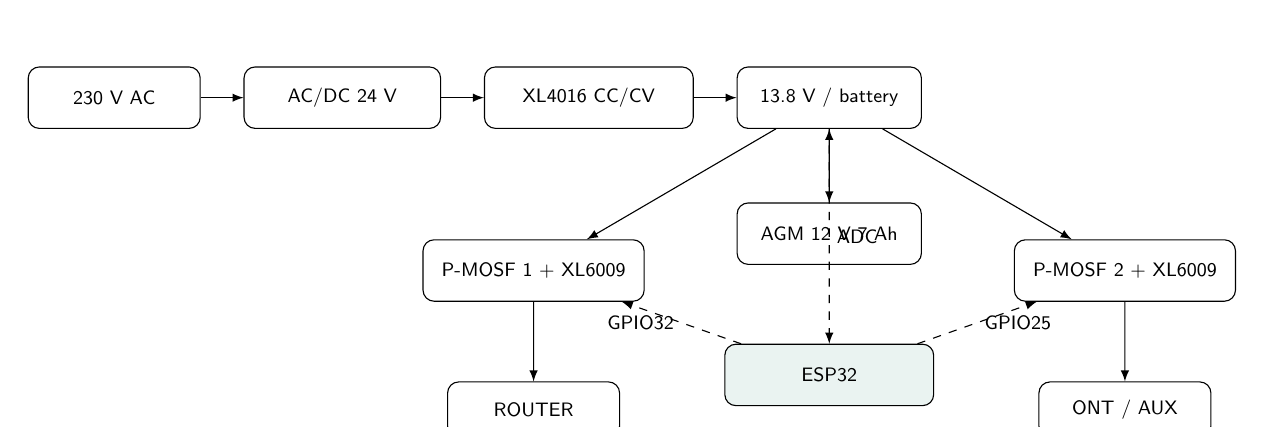
\begin{tikzpicture}[scale=0.78,transform shape,>=latex, node distance=7mm and 7mm, every node/.style={font=\sffamily\small}]
\node[draw,rounded corners,minimum width=28mm,minimum height=10mm] (ac) {230 V AC};
\node[draw,rounded corners,right=of ac,minimum width=32mm,minimum height=10mm] (psu) {AC/DC 24 V};
\node[draw,rounded corners,right=of psu,minimum width=34mm,minimum height=10mm] (chg) {XL4016 CC/CV};
\node[draw,rounded corners,right=of chg,minimum width=30mm,minimum height=10mm] (bus) {13.8 V / battery};
\node[draw,rounded corners,below=12mm of bus,minimum width=30mm,minimum height=10mm] (bat) {AGM 12 V 7 Ah};
\node[draw,rounded corners,below left=18mm and 15mm of bus,minimum width=36mm,minimum height=10mm] (r) {P-MOSF 1 + XL6009};
\node[draw,rounded corners,below right=18mm and 15mm of bus,minimum width=36mm,minimum height=10mm] (o) {P-MOSF 2 + XL6009};
\node[draw,rounded corners,below=13mm of r,minimum width=28mm,minimum height=9mm] (rr) {ROUTER};
\node[draw,rounded corners,below=13mm of o,minimum width=28mm,minimum height=9mm] (oo) {ONT / AUX};
\node[draw,rounded corners,below=35mm of bus,minimum width=34mm,minimum height=10mm,fill=lightaccent] (esp) {ESP32};
\draw[->] (ac)--(psu); \draw[->] (psu)--(chg); \draw[->] (chg)--(bus); \draw[<->] (bus)--(bat);
\draw[->] (bus)--(r); \draw[->] (bus)--(o); \draw[->] (r)--(rr); \draw[->] (o)--(oo);
\draw[->,dashed] (esp)--node[left]{GPIO32}(r); \draw[->,dashed] (esp)--node[right]{GPIO25}(o);
\draw[->,dashed] (bus)--node[right]{ADC}(esp);
\end{tikzpicture}
\end{center}

\subsection{Normal mode}
With mains present the internal AC/DC module produces 24~V. The XL4016 charger steps it down and holds the battery-side bus at the trimmed 13.8~V with a total current limit of 1.5~A. The load and the battery are powered from a shared bus behind a blocking diode according to the specific build.

\subsection{Battery mode}
When the 24~V rail collapses the battery automatically becomes the source for the shared bus. No separate transfer relay is required. The controller detects the mains loss, keeps the enabled channels powered and sends a notification if a network path is available.

\subsection{Deep-discharge protection}
While running on battery the controller compares the battery voltage with the configured thresholds. When LVD is reached both outputs are shut off. Re-enable is not allowed until either the recovery threshold is reached or the mains returns.

After LVD and load release, the controller waits the configured delay and then enters \textbf{emergency deep sleep}. The controller does not wait for a second dip on the unloaded battery ``bounce''. In this mode the ESP32 only wakes on a timer to measure battery voltage and the 24~V rail. Full boot happens only when the mains returns or when the battery recovers above the re-enable threshold.

\subsection{Two sleep modes}
\textbf{Emergency deep sleep} is entered automatically on low battery with the mains absent. Both outputs are off, Wi-Fi is off, the controller wakes on a timer (30~s by default), quickly measures the battery and the 24~V rail, and sleeps again if recovery conditions are not met.

\textbf{Shelf Sleep} is entered only from a long service-button hold. Both outputs, Wi-Fi, mDNS and the setup AP are shut down and the wake-up timer is disabled. The only wake source is the physical button on GPIO14 via EXT0. Restoring 230~V mains \textbf{does not} bring the device out of Shelf Sleep --- the button must be pressed.

% -------------------- 4 --------------------
\section{Controls and indication}

\subsection{LEDs}
\begin{tabularx}{\textwidth}{@{}lX@{}}
\toprule
\textbf{Indicator} & \textbf{Purpose} \\
\midrule
Green, GPIO13 & Indicates external power / mains state \\
Red, GPIO12 & Indicates battery state, warning or emergency mode \\
\bottomrule
\end{tabularx}

Additional patterns:
\begin{itemize}
  \item green blinking at $\approx$2~Hz --- the ESP32 has booted and is trying to join Wi-Fi;
  \item both LEDs alternating slowly (500~ms each) --- the setup AP is active.
\end{itemize}

\subsection{Service button on GPIO14}
The button is wired between GPIO14 and GND. The internal \texttt{INPUT\_PULLUP} is used in normal operation. GPIO14 is chosen because it is also an RTC GPIO usable for EXT0 wake from Shelf Sleep.

\begin{tabularx}{\textwidth}{@{}p{38mm}X@{}}
\toprule
\textbf{Gesture} & \textbf{Function} \\
\midrule
One short press & Send the full current status to the configured ntfy topic. On success the green LED blinks 2 times; if Wi-Fi / ntfy is unreachable the red LED blinks 3 times. \\
Double press & Open \texttt{DC-UPS-Setup} for about 15 minutes. Acknowledged by a short simultaneous flash of both LEDs. \\
Hold for 10~s & Enter Shelf Sleep. Before shutdown the red LED blinks 3 times; then ROUTER and ONT are shut off, Wi-Fi goes down and the ESP32 sleeps with no periodic timer. \\
Press while in Shelf Sleep & Wake the device. The held press is ignored until release, after which a normal start-up runs. \\
\bottomrule
\end{tabularx}

\begin{tcolorbox}[colback=lightwarn,colframe=warn,title=Important: Shelf Sleep]
In Shelf Sleep the device \textbf{does not} wake on the return of 230~V mains. It intentionally stays off until the button is physically pressed. This is a long-term storage / transport mode, not an emergency battery mode.
\end{tcolorbox}

\subsection{Manual output switches}
If separate mechanical switches for ROUTER and ONT are installed on the enclosure, they act as local hardware disconnects for the corresponding output. Their state has priority at the electrical level: software cannot restore power while a mechanical switch is open.

% -------------------- 5 --------------------
\section{Web interface and networking}

\subsection{Access}
With a normal LAN connection the panel is available at:
\begin{center}
\texttt{http://dc-ups.local/}
\end{center}
It is also reachable at the IP address issued by the router. On every successful Wi-Fi connection the firmware may publish the current IP to ntfy.

\subsection{Service access point}
Default SSID: \texttt{DC-UPS-Setup}.\\
Default password: \texttt{dc-ups-setup}.\\
Both parameters can be changed by the owner through the web interface.

\begin{tcolorbox}[colback=lightaccent,colframe=accent,title=Recommendation]
The setup-AP password and the web admin password should not be printed on the outside label. Deliver them separately and change them at commissioning.
\end{tcolorbox}

\subsection{Bidirectional ntfy}
In addition to outgoing notifications the firmware polls the same ntfy topic periodically (roughly every 15~s) and accepts only safe, read-only status commands:
\begin{center}
\texttt{!ups} \qquad \texttt{!ups status} \qquad \texttt{!ups ping}
\end{center}
The \texttt{!ups} and \texttt{!ups status} commands send the full status. The \texttt{!ups ping} command answers with ``PONG'' and the same set of parameters. The reply includes battery voltage, 24~V rail, mains state, ROUTER/ONT, internet, recovery, uptime, outage count, RSSI, IP and the mDNS address.

Remote enable/disable of the outputs through ntfy is \textbf{not implemented} on purpose: the topic is intentionally a read-only status channel. Commands only work while the ESP32 is awake, connected to Wi-Fi and has access to ntfy. In Shelf Sleep and in emergency deep sleep the Wi-Fi radio is off, so commands are unavailable.

\begin{tcolorbox}[colback=lightaccent,colframe=accent,title=ntfy security]
The topic name is effectively a secret URL. Use a long, hard-to-guess name and do not print it on the outside label.
\end{tcolorbox}

\subsection{Available panel features}
\begin{itemize}[leftmargin=7mm]
  \item battery voltage and 24~V rail;
  \item mains presence;
  \item ROUTER and ONT states separately;
  \item ON / OFF / AUTO mode per channel;
  \item independent restart of ROUTER and restart of ONT;
  \item joint restart of both channels;
  \item Wi-Fi state and RSSI;
  \item internet-check state and auto-recovery status;
  \item emergency-sleep state and parameters;
  \item Shelf Sleep and service-button reference;
  \item ADC calibration against a multimeter;
  \item Wi-Fi, ntfy and protection settings;
  \item help on inbound ntfy commands;
  \item event log;
  \item manual ESP32 reboot.
\end{itemize}

% -------------------- 6 --------------------
\section{Automatic connectivity recovery}

The firmware distinguishes between Wi-Fi loss and loss of internet reachability. Typical logic:
\begin{enumerate}[leftmargin=8mm]
  \item If the ESP32 is not associated with Wi-Fi after the allowed waiting period, a reconnect is attempted.
  \item On persistent Wi-Fi failure the ROUTER channel is power-cycled first.
  \item If Wi-Fi is up but the internet is unreachable, the ONT channel is power-cycled first.
  \item On continued failure the next recovery cycle is allowed, including a joint power-cycle of both channels.
  \item The number of automatic power cycles is capped to avoid endless equipment toggling.
  \item After a long period of stable connectivity the auto-recovery counters are reset.
  \item On low battery all automatic power cycles are inhibited to preserve residual charge.
\end{enumerate}

% -------------------- 7 --------------------
\section{Installation and commissioning}

\subsection{Pre-flight}
Before the first power-up or after servicing:
\begin{enumerate}[leftmargin=8mm]
  \item Check the battery polarity.
  \item Check the presence and rating of the battery fuse.
  \item Check that no wires and no live parts are loose.
  \item With a multimeter, set and verify the output voltage of every XL6009 \textbf{before} connecting a load.
  \item Confirm that the DC connector polarity matches the connected equipment.
  \item Confirm that the ROUTER and ONT voltages are recorded in the passport and on the label.
  \item Apply 230~V and check the voltage at the battery terminals.
  \item Verify the mains-to-battery transition by briefly disconnecting 230~V.
\end{enumerate}

\subsection{Acceptance test before handover}
\begin{tabularx}{\textwidth}{@{}XcX@{}}
\toprule
\textbf{Check} & \textbf{Result} & \textbf{Note} \\
\midrule
Battery charge voltage 13.8~V & \yesno & \rule{40mm}{0.4pt} \\
ROUTER ON/OFF/AUTO & \yesno & \rule{40mm}{0.4pt} \\
ONT ON/OFF/AUTO & \yesno & \rule{40mm}{0.4pt} \\
Restart ROUTER from the panel & \yesno & \rule{40mm}{0.4pt} \\
Restart ONT from the panel & \yesno & \rule{40mm}{0.4pt} \\
Mains $\rightarrow$ battery transition & \yesno & \rule{40mm}{0.4pt} \\
LVD & \yesno & \rule{40mm}{0.4pt} \\
Emergency deep sleep and periodic wake-ups & \yesno & \rule{40mm}{0.4pt} \\
Mains return after emergency deep sleep & \yesno & \rule{40mm}{0.4pt} \\
Shelf Sleep: entry by 10~s hold & \yesno & \rule{40mm}{0.4pt} \\
Shelf Sleep: wake only by button & \yesno & \rule{40mm}{0.4pt} \\
Button: 1x status / 2x setup AP & \yesno & \rule{40mm}{0.4pt} \\
Wi-Fi / mDNS & \yesno & \rule{40mm}{0.4pt} \\
ntfy: outgoing notifications & \yesno & \rule{40mm}{0.4pt} \\
ntfy: \texttt{!ups status} / \texttt{!ups ping} & \yesno & \rule{40mm}{0.4pt} \\
Load test on both channels & \yesno & \rule{40mm}{0.4pt} \\
\bottomrule
\end{tabularx}

% -------------------- 8 --------------------
\section{Disassembly and battery replacement}

\begin{tcolorbox}[colback=lightwarn,colframe=warn,title=Hazardous voltage]
Before removing the cover always disconnect the unit from 230~V mains, unplug the mains cord, disconnect the load and open the battery circuit. Even with the mains removed the battery remains an energy source capable of delivering high short-circuit currents.
\end{tcolorbox}

\subsection{Procedure}
\begin{enumerate}[leftmargin=8mm]
  \item Disconnect 230~V and make sure the mains inlet is physically detached.
  \item Turn off the external ROUTER and ONT loads.
  \item Remove the cover following the illustrations in Section~\ref{sec:figures}.
  \item Remove the battery fuse or connector.
  \item First disconnect the terminal called out by the service diagram of the specific build; keep the tool from bridging ``+'' to the case / ``-''.
  \item Disconnect the second terminal and take the battery out.
  \item Install a new AGM/SLA battery 12~V 7~Ah of a compatible size and terminal type.
  \item Connect polarity strictly by the marking: red cable to ``+'', black cable to ``-''.
  \item Reinstall the fuse, check the voltage with a multimeter, and reassemble the enclosure.
  \item Perform a control mains $\rightarrow$ battery transition.
\end{enumerate}

\subsection{Replacement battery requirements}
\begin{itemize}[leftmargin=7mm]
  \item nominal voltage 12~V;
  \item AGM/SLA (sealed lead-acid) technology;
  \item nominal capacity 7~Ah or another value permitted by the enclosure and the charge regime;
  \item compatible dimensions, terminal layout and terminal type;
  \item no bulging, cracks or leakage marks.
\end{itemize}

\subsection{Service images and 3D model}\label{sec:figures}
Assembly views are exported from the public Onshape model (see the 3D-model subsection in the project README). The full STEP files live in \texttt{hardware/enclosure/step/} in the repository.

\realfig{exploded-front.png}{Figure~1. Exploded view --- front side: aluminium extrusion enclosure, AGM 12~V 7~Ah battery installed inside, front panel with IEC~C14 mains inlet, power switch and two DC output receptacles displaced to the left.}

\realfig{exploded-rear.png}{Figure~2. Exploded view --- rear side: enclosure with the controls installed, rear panel removed, two-tier PCB assembly with the XL4016 charger, two XL6009 DC/DC modules and the ESP32 board displayed.}

\blankfig{55mm}{Figure 3. Cover fasteners / clips and disassembly direction}
\blankfig{55mm}{Figure 4. Position of the fuse and battery terminals}
\blankfig{55mm}{Figure 5. Removal and installation of the battery}
\blankfig{55mm}{Figure 6. Close-up of XL4016, ESP32, both XL6009 and the power channels}

% -------------------- 9 --------------------
\section{Maintenance}

Recommended interval: once every 3--6 months, and additionally after any prolonged outage or after the autonomous runtime shortens noticeably.

\begin{itemize}[leftmargin=7mm]
  \item visual inspection of the enclosure and cabling;
  \item check for heat, smell, discoloration or component deformation;
  \item terminal-torque check with the unit de-energised;
  \item battery charge voltage at the terminals;
  \item voltage on both outputs;
  \item battery-mode test;
  \item LVD and recovery test;
  \item check battery condition and installation date;
  \item review the event log and outgoing ntfy notifications;
  \item verify the reply to \texttt{!ups status};
  \item verify Shelf Sleep entry and button wake.
\end{itemize}

\subsection{Expected battery service life}
The life of a sealed lead-acid battery depends on temperature, depth and frequency of discharge and the quality of the float charge. The battery is a consumable and must be replaced when the actual autonomous runtime drops significantly, when the case deforms or when the terminal voltage becomes unstable under load.

% -------------------- 10 --------------------
\section{Troubleshooting}
\begin{longtable}{@{}p{38mm}p{48mm}p{74mm}@{}}
\toprule
\textbf{Symptom} & \textbf{Possible cause} & \textbf{Action} \\
\midrule
\endhead
No power on either output & OFF mode, LVD, missing battery, fuse or shared-bus failure & Check the web panel, battery voltage, fuse and terminals \\
No ROUTER & Channel 1 off, mechanical switch, channel-1 XL6009 or power stage & Check ROUTER mode and voltage before/after the corresponding DC/DC \\
No ONT & Channel 2 off, mechanical switch, channel-2 XL6009 or power stage & Check ONT mode and voltage before/after the corresponding DC/DC \\
Web panel not reachable & ESP failed to join Wi-Fi or the router is off & Use the service button, the setup AP and the serial port for diagnostics \\
Wi-Fi up, no internet & ONT / provider / WAN fault & Check the log; the device may automatically restart ONT \\
Battery discharges fast & Ageing battery or increased load & Measure the load current / power and run a capacity test \\
System went into deep sleep & Low battery after LVD with no mains & Restore 230~V and wait for the next periodic probe \\
Device did not start after 230~V was restored & Shelf Sleep is active & Press the service button; 230~V is intentionally not a wake source in this mode \\
Button caused 3 red blinks & Status could not be sent to ntfy & Check Wi-Fi, internet and topic configuration; the device continues to operate \\
\texttt{!ups status} does not reply & Device is sleeping, no Wi-Fi/internet or wrong topic & Wake the device if necessary; check Wi-Fi and topic; commands are polled about once every 15~s \\
Output voltage sags & XL6009 overload, poor contact, power stage or wiring & Remove the load, measure voltage across the chain, check current and heat \\
\bottomrule
\end{longtable}

% -------------------- 11 --------------------
\section{Package contents}
\begin{tabularx}{\textwidth}{@{}clXc@{}}
\toprule
\# & \textbf{Item} & \textbf{Note} & \textbf{Qty} \\
\midrule
1 & DC-UPS-2CH & Main unit & 1 \\
2 & Battery 12~V 7~Ah AGM/SLA & Installed in the enclosure & 1 \\
3 & Passport and user manual & This document & 1 \\
4 & Warranty card & Part of this document & 1 \\
5 & Output power cables & \rule{55mm}{0.4pt} & \rule{10mm}{0.4pt} \\
6 & Other & \rule{55mm}{0.4pt} & \rule{10mm}{0.4pt} \\
\bottomrule
\end{tabularx}

% -------------------- 12 --------------------
\section{Certificate of acceptance}
The DC-UPS-2CH \hwversion\ unit, serial number \rule{50mm}{0.4pt}, has been assembled, tested and found fit for operation subject to compliance with this manual.

\vspace{5mm}
\begin{tabular}{@{}p{55mm}p{90mm}@{}}
Date of manufacture: & \rule{65mm}{0.4pt} \\
Date of inspection: & \rule{65mm}{0.4pt} \\
Inspected by: & \rule{65mm}{0.4pt} \\
Signature: & \rule{65mm}{0.4pt} \\
\end{tabular}

% -------------------- 13 --------------------
\newpage
\section{Warranty card}

\begin{tcolorbox}[colback=white,colframe=accent,boxrule=1pt,arc=2mm]
\begin{tabular}{@{}p{55mm}p{90mm}@{}}
Product: & DC-UPS-2CH \hwversion \\
Serial number: & \rule{65mm}{0.4pt} \\
Date of transfer: & \rule{65mm}{0.4pt} \\
Manufacturer / integrator: & \rule{65mm}{0.4pt} \\
Owner: & \rule{65mm}{0.4pt} \\
Warranty period: & \rule{30mm}{0.4pt} months \\
\end{tabular}
\end{tcolorbox}

\subsection*{The warranty covers}
Manufacturing defects and internal component failures under compliance with the operating conditions, unless stated otherwise in writing at handover.

\subsection*{The warranty does not cover}
\begin{itemize}[leftmargin=7mm]
  \item natural ageing and capacity loss of the battery;
  \item damage caused by reverse polarity, short circuits or connection of loads with wrong voltage;
  \item overloads beyond the ratings recorded in the passport;
  \item water ingress, condensation, fire, lightning or other external influence;
  \item mechanical damage;
  \item consequences of unauthorised modification of the power section or of settings beyond agreed limits;
  \item faults of the external router, ONT, provider network and connected cabling.
\end{itemize}

\subsection*{Repair record}
\begin{tabularx}{\textwidth}{@{}p{25mm}Xp{35mm}@{}}
\toprule
\textbf{Date} & \textbf{Work performed} & \textbf{Signature} \\
\midrule
\rule{0pt}{10mm} & & \\
\midrule
\rule{0pt}{10mm} & & \\
\midrule
\rule{0pt}{10mm} & & \\
\bottomrule
\end{tabularx}

\vfill
\begin{tabular}{@{}p{72mm}p{72mm}@{}}
Manufacturer's signature: \rule{35mm}{0.4pt} & Owner's signature: \rule{35mm}{0.4pt} \\
\end{tabular}

% -------------------- 14 --------------------
\newpage
\section{Quick reference for the owner}
\begin{enumerate}[leftmargin=8mm]
  \item Under normal conditions no manual switching between mains and battery is needed.
  \item On mains loss operation continues from the battery until the protection threshold is reached.
  \item After LVD the device drops the load and enters emergency deep sleep to preserve the battery.
  \item After mains return the device automatically exits \textbf{emergency} deep sleep, enables the allowed outputs and restores Wi-Fi.
  \item Panel: \texttt{http://dc-ups.local/}.
  \item Button: 1 short --- status to ntfy; 2 shorts --- setup AP for 15 minutes; hold 10~s --- Shelf Sleep.
  \item In Shelf Sleep the device wakes \textbf{only from the button}; restoring 230~V does not turn it on.
  \item Status query through ntfy: \texttt{!ups}, \texttt{!ups status} or \texttt{!ups ping}.
  \item Before connecting new equipment verify the required voltage and polarity.
  \item Do not open the enclosure while 230~V mains or the battery is connected.
\end{enumerate}

\begin{center}
\vfill
\qrcode[height=28mm]{http://dc-ups.local/}\\[2mm]
{\small Quick jump to the local panel (works from the same LAN with mDNS support).}
\end{center}

\end{document}
